
These results are based on the assumptions that the $Np$ informed individuals are guiding and moving in front of the rest, that they move in a circle making a quadratic bounding box around them, and that all individuals maintain a homogenous density with distance $\alpha$ to each other. This justifies the approximation illustrated in Figure \ref{fig:distr}. There will effectively be $Np\omega$ guiding individuals if the weight $\omega$ is taken into account. Figure \ref{fig:guiding} shows how the individuals are moving in the simulation at time $t=500$.

\begin{figure}[H]
\begin{center}
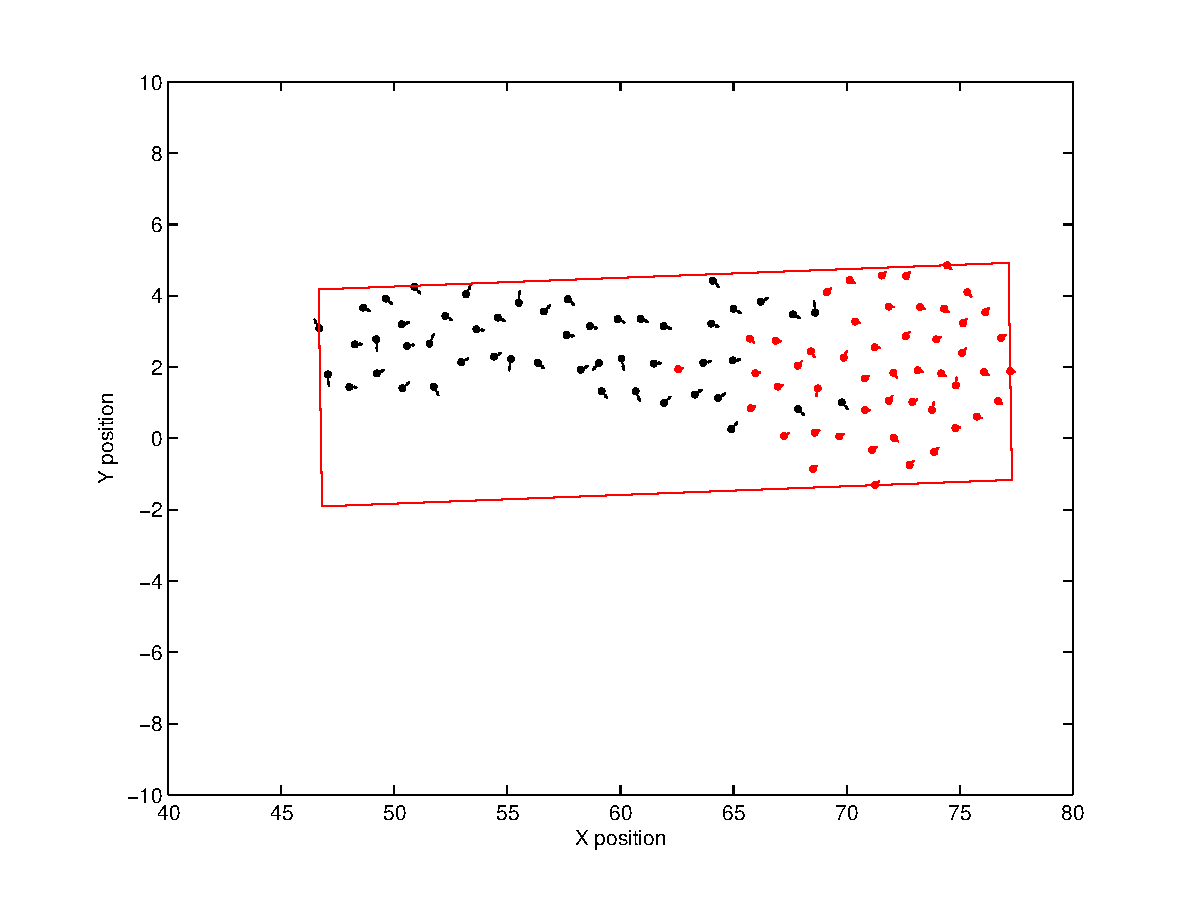
\includegraphics[width=\linewidth]{img/guiding.eps}
\caption{The informed individuals (red markers) are guiding the rest of the group. Parameters used are $\omega = 0.5$, $p = 0.5$, and N=100.}
\label{fig:guiding}
\end{center}
\end{figure}

\newcommand{\figwidth}{0.21\textwidth}
\begin{figure}[H]
	\centering
	\begin{subfigure}[b]{\figwidth}
		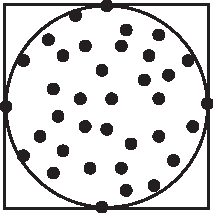
\includegraphics[width=\textwidth]{img/Circle.pdf}
		\caption{Actual distribution in box.}
		\label{fig:distr_true}
	\end{subfigure}
	~
	\begin{subfigure}[b]{\figwidth}
		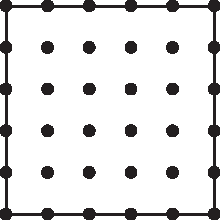
\includegraphics[width=\textwidth]{img/Square.pdf}
		\caption{Approximated distribution.}
		\label{fig:distr_approx}
	\end{subfigure}
	\caption{Approximation of particle distribution inside bounding box.}
	\label{fig:distr}
\end{figure}

\begin{figure}[H]
	\centering
	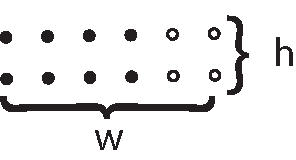
\includegraphics[width=0.24\textwidth]{img/heightwidth.pdf}
	\caption{Assumption of distribution when 4 out of 12 particles have information of destination. Circles indicates informed particles, solid dots indicates uninformed.}
	\label{fig:distr_direction}
\end{figure}
From the definition of Elongation, see section \ref{sub:elongation}, we can formulate an approximation of the elongation that is valid when the informed individuals have enough influence to guide the rest. With a distance between particles of length $\alpha$ we can define the parameters in Figure \ref{fig:distr_direction} as
\begin{align}
	h &= (\sqrt{Np\omega}-1)\alpha \\
	w & = (\frac{N}{\sqrt{Np\omega}} -1) \alpha.
\end{align}
The elongation is calculated as 
\begin{equation}
	E = \frac{w}{h} = \frac{(\frac{N}{\sqrt{Np\omega}} -1)}{\sqrt{Np\omega}-1}.
\end{equation}
For large $N$, the elongation can be approximated by
\begin{equation}
	E \approx \frac{1}{p\omega}.
\end{equation}